%  Pt2.tex
% !TeX spellcheck = en_GB
% !TeX root = ProjectRiskManagement.tex

\section{Identify \textit{All} the Relevant Sources of Uncertainty} \label{s:Identify}
%\todo{900 Words}

% the identify phase of the PUMP approach, in the execution and delivery strategy shaping phase of a project’s lifecycle, explain concisely in your own words what you believe are the key features of a PUMP approach, comparing these features with the PMI PIMBOK approach or any other form of common practice you are familiar with. Your discussion should demonstrate your ability to understand a particular area of the course material in depth, based on selective reading, critical analysis and the case study exercise. Use examples to illustrate your discussion if you wish, making use of the Samdo case study if you wish, but concentrate on concepts and principles. Build on your Part 1 answer, avoiding repetition of earlier discussion.
%900words.

%Key Features

%Compare with PMI PMBOK or others

%In depth understanding

The identify phase is common through several risk management methodologies, including PUMPs. 
However, there is a marked removal from common practice in the PUMP approach resulting in an iterative, holistic, inherently creative methodology to identify all relevant sources of uncertainty, possible response options, assumptions, conditions and second-order sources.
This encourages the consideration of all types of uncertainty to a relevant degree of detail thus achieving clarity efficiency.

Common practice approaches such as the Project Risk Management (PRM) framework prescribed by the Project Management Institute \citep{pmi2013} are linear processes whereby all relevant risk events must be identified at an early stage. 
The identification of response options is left until later in the linear process and decoupled from the identification of the sources themselves.
Assumptions and conditions are also decoupled, since unbiased estimation is not a formal goal of the process. 
This approach does not optimise clarity efficiency and powerful general responses are often not realised until a much later stage.
The complexity relating to secondary sources of uncertainty due to the consequences of response options is not considered.
Moreover, a dangerous false sense of security can be created through such approaches where linearity obscures the underlying complexity which may ultimately endanger the achievement of project objectives.
                         
Within the PUMP framework, the identification of sources of uncertainty and possible response options are closely coupled. 
Considering possible response options as new sources are identified increases the chances of developing powerful general responses that are critical to the delivery of clarity efficiency. 
Moreover, unidentified responses contribute to ambiguity uncertainty. 
On some occasions the consequences of the response can lead to secondary sources which may also require consideration.
The identify phase allows an enlightened reshaping of relevant base plans and contingency plans as required.

\begin{figure}[!h]
  \centering
    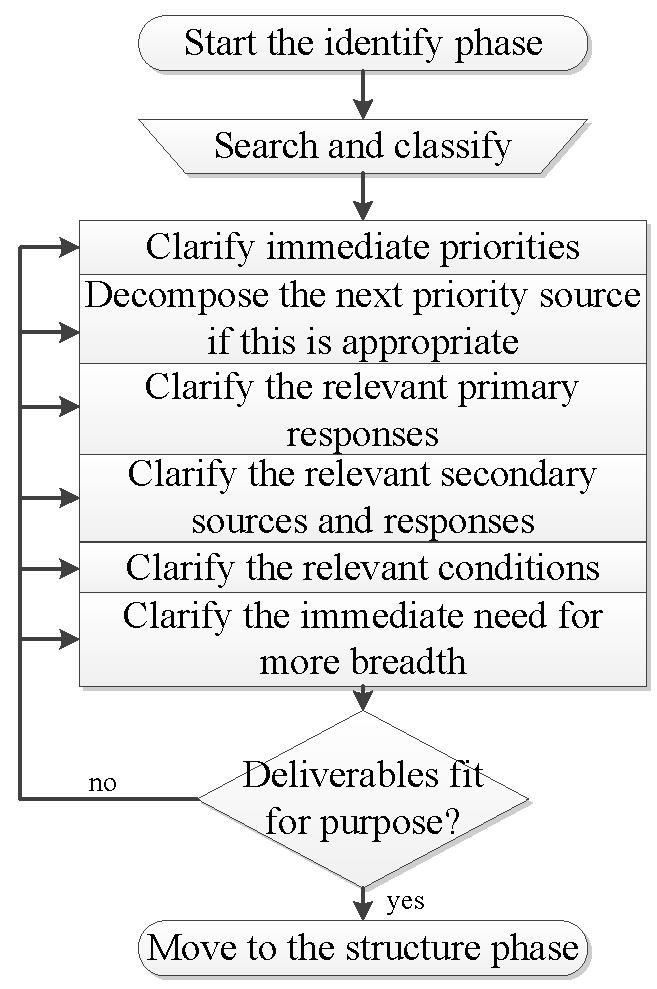
\includegraphics[width = 0.41\textwidth]{./Figures/Identify.png} 
\caption{Identify Phase Process - adapted from \cite{chapman}}
\label{Figure:Identify}
\end{figure}

The process has two main features. 
The \textbf{search} task involves finding all relevant sources responses and conditions. 
The \textbf{classify} task provides a suitable structure where sources have been aggregated or decomposed as necessary upon which further analysis can proceed.
The process is shown in figure \ref{Figure:Identify}.
The keyword in the process is `relevant'. 
The skill of the risk practitioner is in seeing where maintaining strategic level composite sources or decomposing to further levels of detail is useful.

The search for relevant response options is addressed in step 2 of figure \ref{Figure:Identify}.
An informal assessment of each response option is required which is usually easiest when the uncertainty types are viewed as a general composite.
The search for possible responses is simple at face value.
Following the identification of a source of uncertainty, it is frequently obvious how one would immediately respond.
However, a more considered systematic approach may uncover opportunities that are not immediately apparent, particularly for sources that are particularly significant or complex.

The \citet{pmi2013} advocates four generic response types; avoid, transfer, mitigate and accept.
Figure \ref{Figure:ResponseTypes} shows eleven generic response options that \citet{chapman} assimilate from literature.
The mind-map format indicates that this is by no means a complete list of responses, but a trigger for the consideration of diverse response options.
In reality, many responses fall into several categories.
The aim of using such tools in this step is to maximise opportunity efficiency through robust early response development and a qualitative understanding of the consequences. 
This enables important sources of risk inefficiency to be designed out and provides a clarity efficient methodology for capturing opportunities.

\begin{figure}[!h]
  \centering
    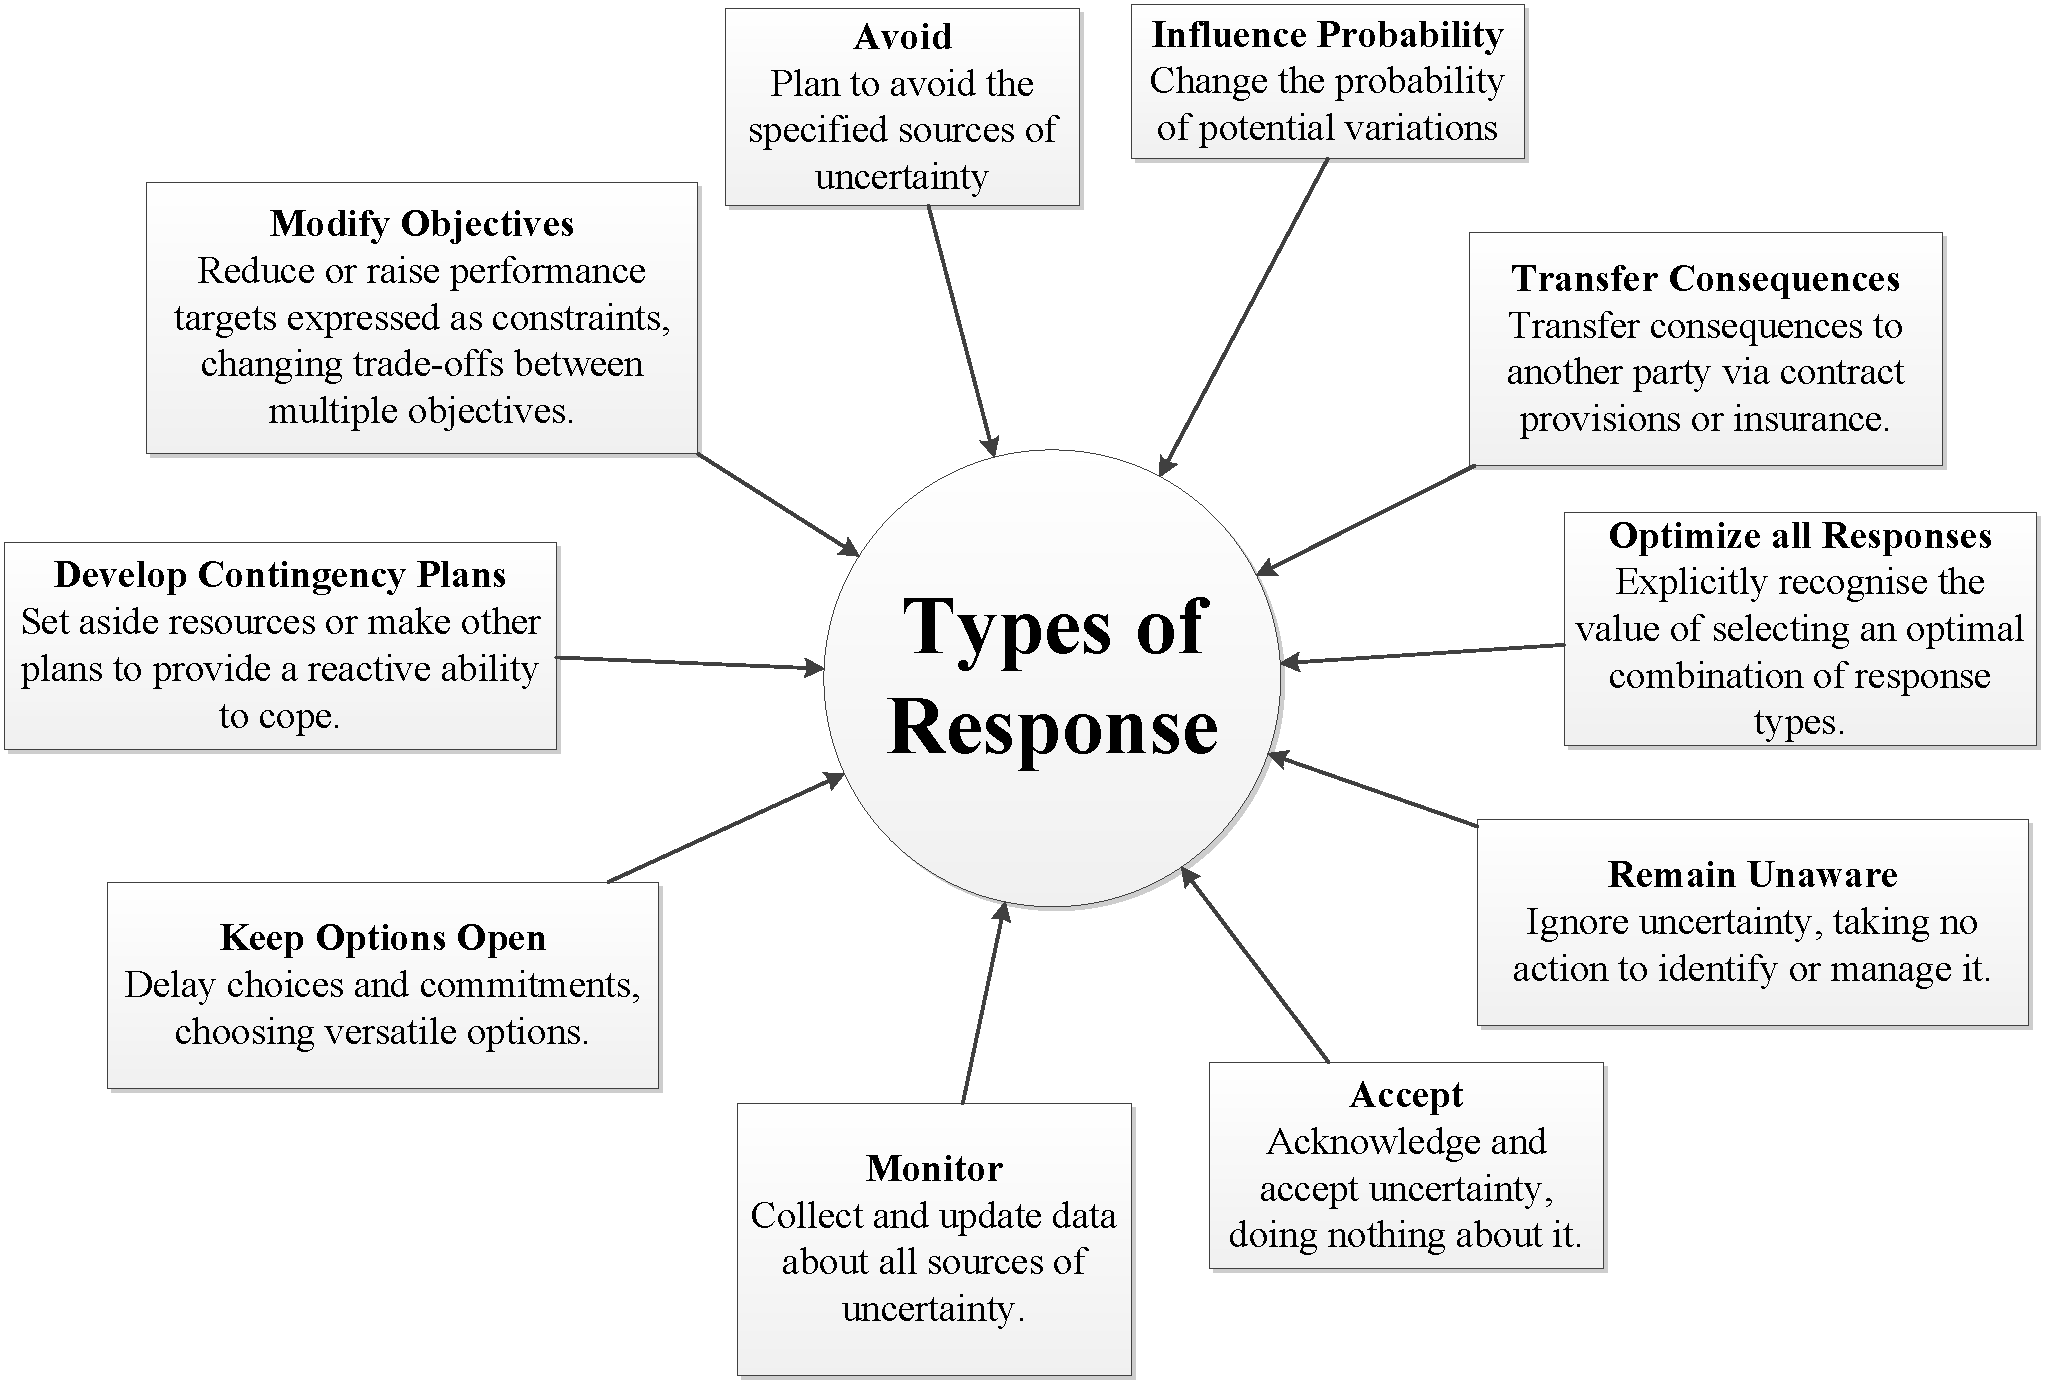
\includegraphics[width = \textwidth]{./Figures/ResponseTypes.png} 
\caption{Generic response types - adapted from \cite{chapman}}
\label{Figure:ResponseTypes}
\end{figure}

For the identify phase to be effective, creativity must be embraced and encouraged.
Identification can be undertaken by an individual or by a team of practitioners.
The most straightforward approaches are 'pondering' techniques using a simple blank sheet of paper.
While this could prove too simple and limited for some projects, it should not be dismissed as a starting point.
Brainstorming is another familiar technique used to harness creativity.
When used with groups with particularly keen understanding of the project at hand, or those with applicable prior experience, brainstorming can provide important responses.
Synectics \citep{gordon1961synectics} and decision-conferencing techniques \citep{finlay1991review} are alternative techniques for problem-solving with groups of people.
List based approaches could also prove useful as checklists to ensure the creative process has considered viable alternatives before moving on.
Encouraging creative solutions and harnessing the relevant experience and expertise in a clarity efficient manor is key to realising powerful general response options and uncovering key opportunities.


Special consideration of the identify phase has been given in this report, since when operating in a high clarity context, identification can require significant effort.
However, given an understanding of the process and of the project at hand, it is arguably one of the simplest phases in the PUMP framework.
Simplification for lower levels of clarity is possible, providing the balance between clarity efficiency and holistic consideration is maintained.
Clarity efficiency remains the key principle.
The identify phase must ensure an adequate level of decomposition is performed for important sources, while higher level aggregates are utilised for those less important.
The common practice approach offers only a glimpse of the total uncertainty, often missing key opportunities and the underlying complexities of sources identified.
The PUMP approach to identification gives the widest possible appreciation of uncertainty as early as practicable in the process, which allows risk efficiency and most importantly opportunity efficiency to be achieved.


\clearpage






